\documentclass[11pt]{scrartcl}
\usepackage[utf8]{inputenc}
\usepackage{amsmath, amssymb, amsthm, bbm}
\usepackage{booktabs, verbatim, graphicx, framed}
\usepackage[sexy, hints]{evan}
\title{Physics Homework With Greenwood, Chapter 4}
\author{Anay Aggarwal}

\begin{document}

\maketitle
\begin{example}
  [Context-Rich Problem]
  Gymnast
\end{example}
\begin{soln}
To solve this problem, we'll need to know about forces. Specifically,
we'll need to know that
$$\sum \overrightarrow{F}=m\overrightarrow{a}$$
We'll also need to know basic trig.
\\ \\
Assume that upwards is positive $y$, and rightward is positive $x$.
Let $G$ be the gymnast, $E$ be the Earth, $T$ be tension, $R_1,R_2$ be the ropes, and $g$ be gravity.
The freebody diagram is the following:
\begin{center}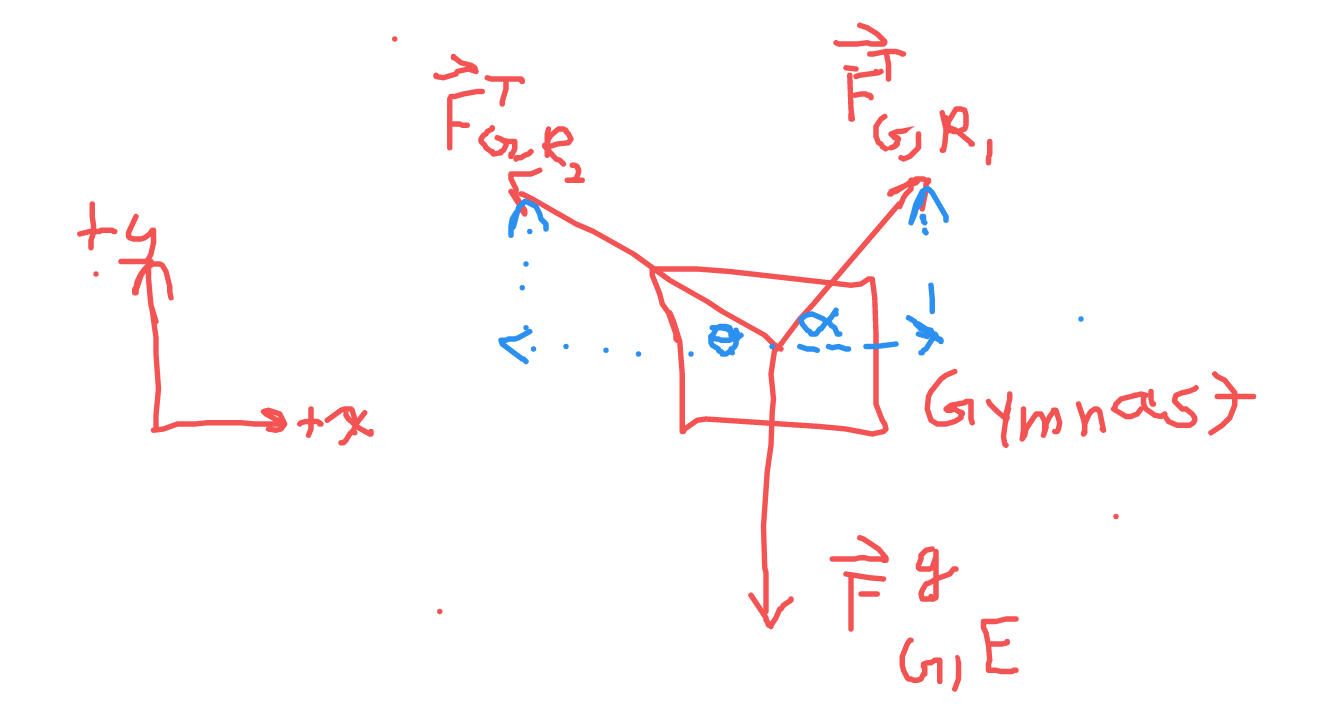
\includegraphics[scale=0.3]{impostor.png}\end{center}
Since we have forces in various directions, it will likely be helpful to split the force
vectors into their components. The components (using the diagram), are the following:
$$\overrightarrow{F_{G,R_2}^T}=-F_{G,R_2}^T\cos\theta \hat{x}+F_{G,R_2}^T\sin\theta \hat{y}$$
$$\overrightarrow{F_{G,R_1}^T}=F_{G,R_1}^T\cos\alpha\hat{x}+F_{G,R_1}^T\sin\alpha \hat{y}$$
Keeping the signs in mind. Notice that there is no total acceleration, so
$$\sum \overrightarrow{F}=m\overrightarrow{a}=0$$
Therefore,
$$(F_{G,R_1}^T\cos\alpha-F_{G,R_2}^T\cos\theta)\hat{x}+(F_{G,R_1}^T\sin\alpha+F_{G,R_2}^T\sin\theta-F_{G,E}^g)\hat{y}=0$$
This equation tells us a lot of things, since both the x and y components of the vector are equivalent to $0$.
This gives us two separate equations:
$$F_{G,R_1}^T\cos\alpha-F_{G,R_2}^T\cos\theta=0$$
$$F_{G,R_1}^T\sin\alpha+F_{G,R_2}^T\sin\theta-F_{G,E}^g=0$$
For convenience, denote
$$F_{G,R_1}^T\equiv T_1$$
$$F_{G,R_2}^T\equiv T_2$$
Hence
$$T_1\cos\alpha=T_2\cos\theta\implies T_2=\frac{T_1\cos\alpha}{\cos\theta}$$
$$T_1\sin\alpha+T_2\sin\theta=F_{G,E}^g$$
We know that $F_{G,E}^g=mg$, Therefore,
$$T_1\sin\alpha+T_2\sin\theta=T_1\sin\alpha+T_1\cos\alpha\tan\theta=T_1(\sin\alpha+\cos\alpha\tan\theta)=mg$$
$$\boxed{T_1=\frac{mg}{\sin\alpha+\cos\alpha\tan\theta}}$$
$$\boxed{T_2=\frac{mg\cos\alpha}{\sin\alpha\cos\theta+\cos\alpha\sin\theta}}$$
\\ \\
The units check out since $T_1,T_2$ are forces and their values are a scalar multiplied by force, which is a force.
\\
To check limiting cases, let's fix $\theta$ and play with $\alpha$. When $\alpha\to \frac{\pi}{2}$, $T_1\to mg$ and $T_2\to \frac{mg}{\cos\theta}$, which makes sense (more force required).
When $\alpha\to 0$, $T_1\to \frac{mg}{\tan\theta}$ and $T_2\to \frac{mg}{\sin\theta}$. This also makes sense since $\tan\theta$ can get large or small.
When $\alpha\to\theta$, we get $T_1\to T_2\to \frac{mg}{2\sin\theta}$ which is what we got in class.
\end{soln}
\begin{example}
  [Example Problem]
  Block on ramp
\end{example}
\begin{soln}
  To solve this, we need to know about free-body diagrams and Newton's second law:
  $$\sum \overrightarrow{F}=m\overrightarrow{a}$$
  \\ \\
  For the first part, we can simply apply Newton's second law, which can be rewritten as
  $$\overrightarrow{F}_{net}=m\overrightarrow{a}$$
  Now, the blocks are at rest, hence
  $$\overrightarrow{F}_{net,both}=m\cdot 0=0$$
  Hence both net forces are zero, so the answer is $\boxed{\text{equal to}}$.
  \\ \\
  For the second part, we will need to draw some free-body diagrams. $N$ denotes normal force, $f_s$ denotes static frictional force, $\text{ext}$ denotes external
  force, and $G$ denotes gravitational force.
  \begin{center}
    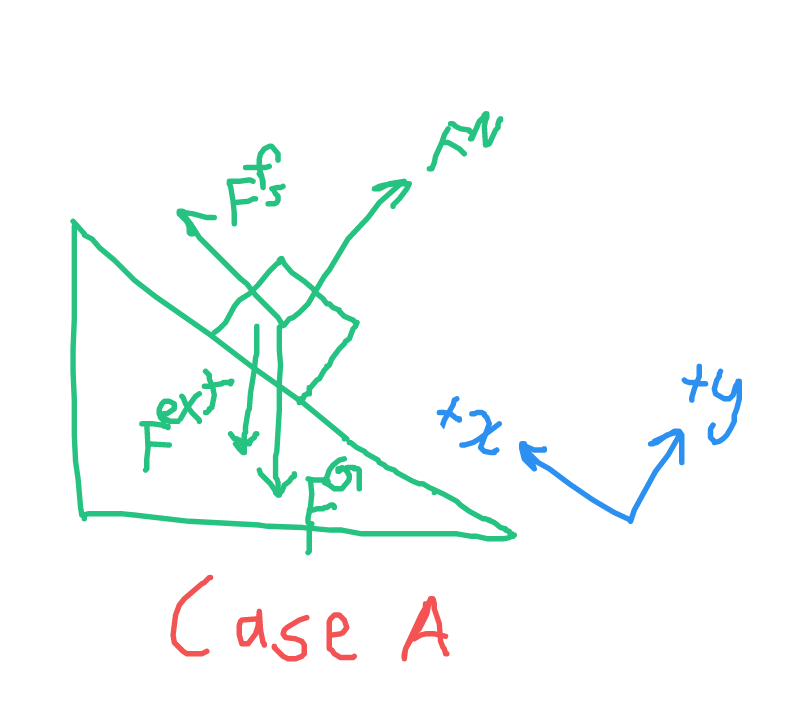
\includegraphics[scale=0.3]{CaseA.png}
    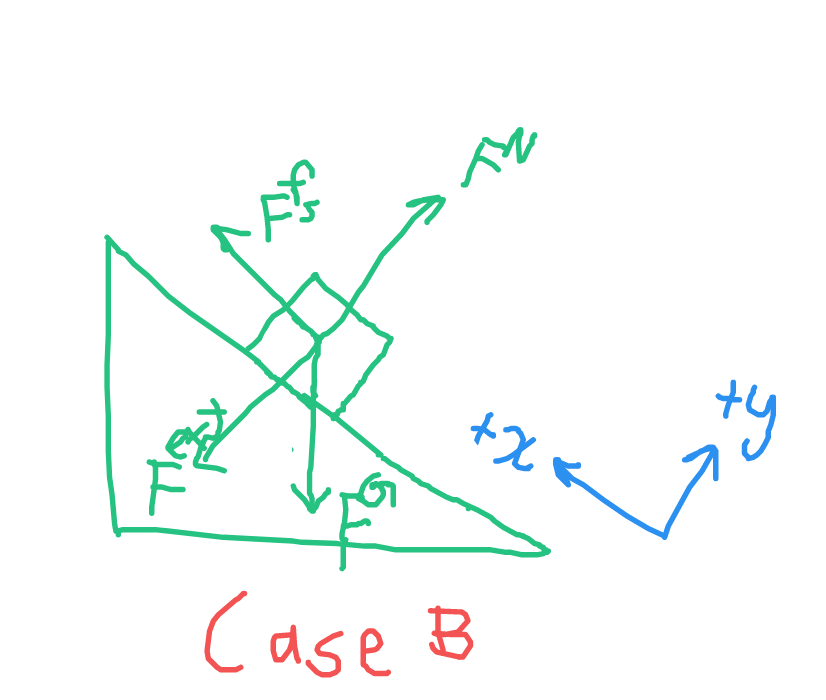
\includegraphics[scale=0.3]{CaseB.png}
  \end{center}
  Notice that the axes are along the plane (for convenience). Now, I claim that
  the frictional force in Case A is greater than in Case B. To show this, notice that by Newton's
  second law, the forces sum to $0$. In Case A, the only forces in the x-direction are:
  \begin{itemize}
    \item Positive static frictional force
    \item Negative x-component of gravity
    \item Negative x-component of external force
  \end{itemize}
  And for Case B:
  \begin{itemize}
    \item Positive static frictional force
    \item Negative x-component of gravity
  \end{itemize}
  Noting that the x-components of gravity are equal since the angles and masses are equal,
  the frictional force in Case A has to make up for gravity \textit{and more}, whereas
  Case B only has to make up for gravity (since the external force in this case is in the y-direction).
\end{soln}
\end{document}
